\fancychapter{Introduction}
\cleardoublepage%
% The following line allows to ref this chapter
\label{chap:intro}%



\section{Motivation}
 
% \par Worldwide, there has been growing interest in the use of autonomous vehicles to execute missions of increasing complexity without constant supervision of human operators.~\cite{xargay2012time} A key-enabling element for the execution of such missions is the availability of advanced methods for cooperative motion planning that take explicitly into account temporal and spatial constraints, intrinsic vehicle limitations and energy minimisation requirements. 
% \par Some autonomous vehicle applications require groups of robots acting cooperatively. An application example that will greatly benefit from vehicle cooperation and that will be focus of this thesis is the control of groups of \acp{AUV} where the visibility is low and obstacles are not known in advance. The \acp{AUV} that together form a robot formation, can, for example, adapt better to unforeseen circumstances in the terrain by making better use of the larger environments that they can observe as the spatial distance between each \ac{AUV} can be varied.
% \par This project has evolved from earlier investigations on underwater mapping connected with the European R\&D Project "MORPH" Project~\cite{morph,aguiar2009cooperative,abreu2016widely} that Insitituto Superior Técnico was a part of. Figure~\ref{fig:morph} illustrates \acp{AUV} in operation on the Morph project.


\par Worldwide, there has been growing interest in the use of autonomous vehicles to execute missions of increasing complexity without constant supervision of human operators.~\cite{xargay2012time} A key-enabling element for the execution of such missions is the availability of advanced methods for cooperative motion planning that take explicitly into account temporal and spatial constraints, intrinsic vehicle limitations and energy minimisation requirements. 
\par Some autonomous vehicle applications require groups of robots acting cooperatively. An application example that will greatly benefit from vehicle cooperation and that will be focus on this thesis is the control of groups of \acp{AUV} where the visibility is low and obstacles are not known in advance. The \acp{AUV} that together form a robot formation, can, for example, adapt better to unforeseen circumstances in the terrain by making better use of the larger environments that they can observe as the spatial distance between each \ac{AUV} can be varied.
\par This project has evolved from earlier investigations on underwater mapping connected with the European R\&D Project "MORPH" Project~\cite{morph,aguiar2009cooperative} and the "WiMUST" Project~\cite{abreu2016widely} that Insitituto Superior Técnico was a part of. Figure~\ref{fig:morph} illustrates \acp{AUV} in operation on the Morph project.
\par The "WiMUST" project, in particular, was composed by a small fleet of \acp{AUV} towing streamers with hydrophones to acquire sub-bottom profiling acoustic data.
\par Recent advancements on the usage of \textit{Bernstein Polynomials} for control also appear to be advantageous,~\cite{cichella2018bernstein}, shows that it's possible to control a high number of vehicles with small computation time.

\begin{figure}[h!]
    \centering
    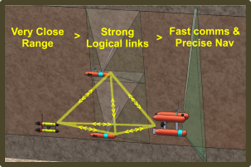
\includegraphics[width=0.5\textwidth]{Images/projects/Picture2.png}
    \caption{Morph Project}
    \label{fig:morph}
\end{figure}
    
\begin{figure}[h!]
    \centering
    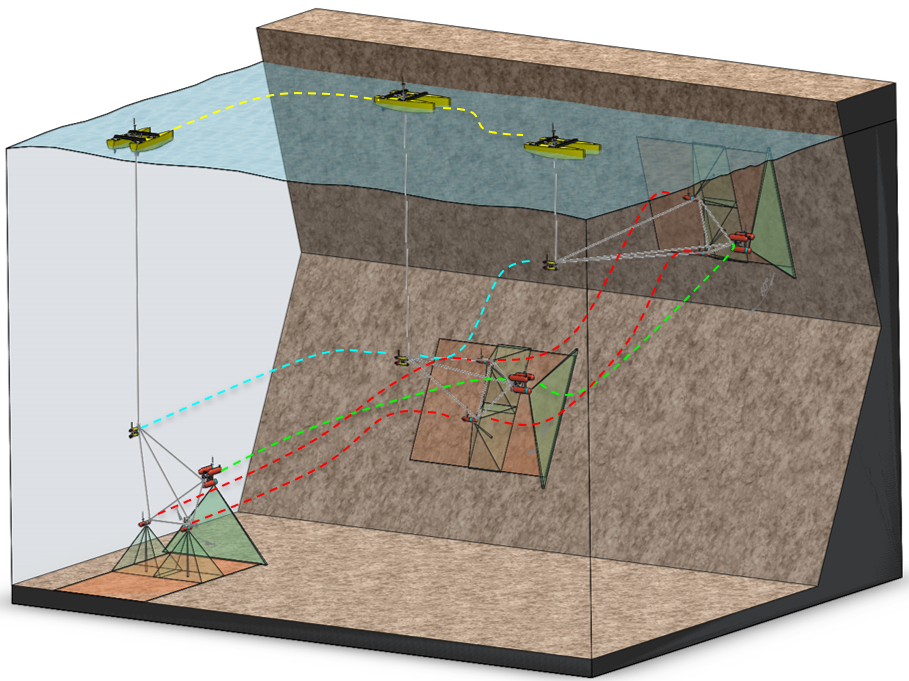
\includegraphics[width=0.6\textwidth]{Images/projects/Picture1.png}
    \caption{Morph Project}
    \label{fig:morph}
\end{figure}


\section{Background}

\par The work discussed in this thesis emphasises in the use of motion planning for multiple cooperative vehicles. Motion Planning, as the name suggests, consists in planning motion for robots, such as mobile vehicles or robotic arms. The choice of control law, i. e., the input which is provided to a robot, will result in a motion which is optimal according to a certain criteria. This criteria could be, for example, minimising time or consumed fuel. Formulisation of such a problem is known as an optimal control problem.
\par There are two main families of techniques for solving optimal control problems: direct methods and indirect methods.
\par In an indirect method, the calculus of variations is employed to obtain the first-order optimality conditions. These conditions result in a two-point (or, in the case of a complex problem, a multi-point) boundary-value problem.

% https://math.stackexchange.com/questions/946343/optimal-control-difference-between-indirect-direct-approaches
\par Direct methods in optimal control convert the optimal control problem into an optimization problem of a standard form and then using a nonlinear program to solve that optimization problem. 
\par In direct approaches the optimal control problem is transfonned into a nonlinear
programming problem.
\par In a direct method, the state or the control, or both, are paramaterized in order to create an appropriate function approximation (e.g., polynomial approximation or piecewise constant parameterization). Simultaneously, the cost functional is approximated as a cost function. Then, the coefficients of the function approximations are treated as optimization variables and the problem is "transcribed" to a nonlinear optimization problem.

\par A path is a parameterized curve, which is a function that maps a segment $[a,b]$ to $\mathbb{R}^3$. If the parameter of path $p$ is time or a function of time, the map $t\mapsto p(t)$ is called a trajectory.
\par \ac{PF} refers to the problem of making vehicles converge to and follow a path with no explicit temporal schedule while \ac{TT} is the problem of making a vehicle track a trajectory such that both spacial and temporal schedules are satisfied simultaneously.
\par Motion Planning consists in the design of trajectories for different kinds of systems that can later be tracked.
\par A trajectory is the path that an object with mass in motion follows through space as a function of time. Trajectory tracking is the 
\par The objective of motion planning is to find a trajectory to be tracked by a robot in an optimal way, based on a "cost function".

\par Once decided what kind of parameterization will be used, the next step is to choose what model to represent the vehicle. Different models to represent vehicles exist such as a Dubin's car, Medusa Model.
% \par There are two main strategies for motion planning, one is \ac{TT} and the other is \ac{PF}. The first requires a vehicle to follow a path parameterized in space and time, whereas the latter only requires the vehicle to follow a path parameterized in space. Regardless of the strategy, the resulting evirnomental and dynamic constraints are met. Environmental constraints may include inter vehicular constraints, obstacle avoidance. Dynamic constraints include respecting maximum torque, acceleration, velocity and others for each vehicle.



\section{Objectives}


\par The work presented in this thesis focuses on the useage of Direct Methods.
\par There are several direct methods for trajectory optimisation, for example, single and multiple shooting, collocation and quadratic programming. However, polynomial methods based on Bezier curves are particularly advantageous because they have favourable geometric properties which allow the efficient computation of the minimum distance between trajectories. As the complexity of the polynomials increases, the solutions converge to the optimal.
\par The cost can be constructed based on several criteria such as time and consumed energy. For \textit{cooperative} motion planning, the cost will have to be constructed differently because it will have to take into account the motion of the multiple vehicles at once, in particular, possible inter-vehicle collision.

\begin{itemize}
    \item test some methods for obstacle avoidance
    \item compare some different parameterization methodoligies
    \item analize the complexity of increasing order and number of vehicles
\end{itemize}

\todo{explain that we want to show that bernstein methods work for non differentially flat models like medusa}

\par The usage of log barrier functions may help with speedinng up the optimisation process because they reduce the number of constraints by placing them in the cost function.



% https://en.wikipedia.org/wiki/Optimal_control


\section{Thesis Outline}


% to use refs: \ref{chap:available_methods} try \Cref{} too. it works for more than just  chapters
\par In chapter \ref{chap:theory}, an overview of the different available numerical methods for the motion planning for a single vehicle will be presented. \todo{exapnd}
\par In chapter \ref{chap:autonomousvehiclemodels}, an overview of different vehicle models is presented. \todo{expand}
\par In chapter \ref{chap:implementation}, a discussion of the code structure is discussed, along with the choice of optimisation algorithms. \todo{exapnd}
\par In chapter \ref{chap:results}, some results are presented. \todo{exapnd}
\par In chapger \ref{chap:conclusion}, the conclusion is made. \todo{exapnd}

This will be followed, in chapter , by application examples for a double integrator in 1 and 2 dimensions that capture the dynamics of a single vehicle. In chapter , some considerations for the control of multiple cooperative vehicles will be presented. The report will be concluded with a final overview of the different methods considered and a plan for the project's work will be defined.
